% This text is proprietary.
% It's a part of presentation made by myself.
% It may not used commercial.
% The noncommercial use such as private and study is free
% Sep. 2005 
% Author: Sascha Frank 
% University Freiburg 
% www.informatik.uni-freiburg.de/~frank/


\documentclass[xcolor=table]{beamer}
\usepackage{beamerthemeshadow}
\usepackage{helvet}
\usepackage[]{graphicx}
\usepackage{array}
\usepackage{color}
\definecolor{dkgreen}{rgb}{0,0.6,0}
\definecolor{gray}{rgb}{0.5,0.5,0.5}
\definecolor{mauve}{rgb}{0.58,0,0.82}
\definecolor{deepblue}{rgb}{0,0,0.5}
\definecolor{deepred}{rgb}{0.6,0,0}
\definecolor{deepgreen}{rgb}{0,0.5,0}
\definecolor{lightgray}{rgb}{0.92,0.92,0.92}
\usepackage{listings} % to insert code
\usepackage{textpos} % textblock
\usepackage{hyperref}
\hypersetup{colorlinks=true, urlcolor=blue, linkcolor=black} 
% Listing set up
% bash
\lstdefinestyle{bash}{
language=bash,                     % the language of the code
basicstyle=\scriptsize\ttfamily,       % the size of the fonts that are used for the code
numbers=none,%left,                   % where to put the line-numbers
numberstyle=\tiny\color{gray},  % the style that is used for the line-numbers
stepnumber=1,                   % the step between two line-numbers. If it's 1, each line
                          % will be numbered
numbersep=5pt,                  % how far the line-numbers are from the code
backgroundcolor=\color{lightgray},  % choose the background color. You must add \usepackage{color}
showspaces=false,               % show spaces adding particular underscores
showstringspaces=false,         % underline spaces within strings
showtabs=false,                 % show tabs within strings adding particular underscores
frame=lines,%single,                   % adds a frame around the code
rulecolor=\color{black},        % if not set, the frame-color may be changed on line-breaks within not-black text (e.g. commens (green here))
tabsize=2,                      % sets default tabsize to 2 spaces
captionpos=b,                   % sets the caption-position to bottom
breaklines=true,                % sets automatic line breaking
breakatwhitespace=false,        % sets if automatic breaks should only happen at whitespace
title=\lstname,                 % show the filename of files included with \lstinputlisting;
                          % also try caption instead of title
keywordstyle=\color{blue},      % keyword style
commentstyle=\color{dkgreen},   % comment style
stringstyle=\color{mauve},      % string literal style
escapeinside={\%*}{*)},         % if you want to add a comment within your code
morekeywords={}            % if you want to add more keywords to the set
}

% Python
\lstdefinestyle{python}{
language=python,
formfeed=\newpage,
basicstyle=\scriptsize\ttfamily,
commentstyle=\color{deepgreen},%\color{gray},
numbers=left,
numberstyle=\tiny\color{gray},
stepnumber=1,
numbersep=5pt,
backgroundcolor=\color{lightgray},%\color{white},
showspaces=false,
showstringspaces=false,
showtabs=false,
frame=lines,
tabsize=4,
captionpos=b,
breaklines=true,
breakatwhitespace=false,
title=\lstname,
escapeinside={},
keywordstyle=\color{deepblue},
emphstyle=\color{deepred},
stringstyle=\color{deepgreen}
%morekeywords={models, lambda, forms}
}


\graphicspath{ {../img/} }

\begin{document}
\title{Python for Scientific Research}   
\author{Bram Kuijper} 
\date{\today} 

\frame{\titlepage} 


\frame{
    \frametitle{Course Schedule} 
    \begin{itemize}
        \item Today, March 6: The basics of programming in Python
            \begin{itemize}
                \item how to run Python code
                \item data types
                \item variable scope
                \item flow control
                \item text manipulation
            \end{itemize}
            \pause
        \item March 20th: Applying Python to simplify your life
            \begin{itemize}
                \item functions
                \item working with files
                \item working with data using \texttt{pandas} and \texttt{scipy}
                \item making graphs using \texttt{matplotlib}
            \end{itemize}
            \pause
        \item March 27th: Advanced subjects
            \begin{itemize}
                \item object-oriented programming
                \item automating tasks in MS-office
                \item image manipulation
                \item working on student-generated problems
            \end{itemize}
    \end{itemize}
}

\frame{
    \frametitle{Today's schedule} 
    \begin{itemize}
        \item 1300 - 1400: How to run Python \& Data types
        \item 1400 - 1420: Break
        \item 1420 - 1520: Variable scope \& Flow control
        \item 1520 - 1540: Break
        \item 1540 - 1640: Functions, working with files 
    \end{itemize}
}

\frame{\frametitle{What is Python?}
\begin{itemize}
    \item A scripted, high-level programming language created by Guido Van Rossum and named after Monty Python's flying circus
\begin{center}
    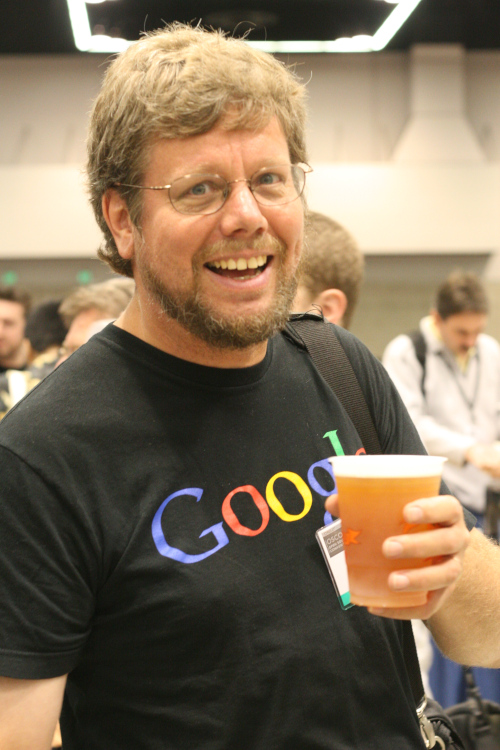
\includegraphics[width = 20mm]{GuidoVanRossumSmall.jpg}
    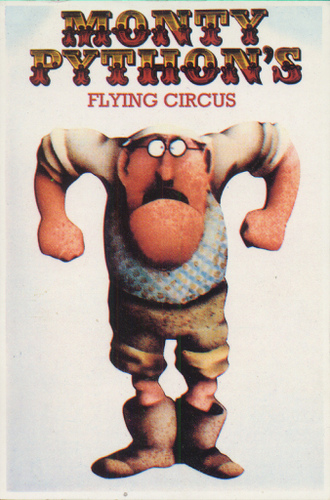
\includegraphics[width = 20mm]{MontyPython.jpg}
\end{center}
    \pause
    \item easy-to-use, highly standardized and with an emphasis on readability of code
\end{itemize}
}


\frame{\frametitle{Why use Python?}
The TIOBE index is a measure of the popularity of programming languages:
    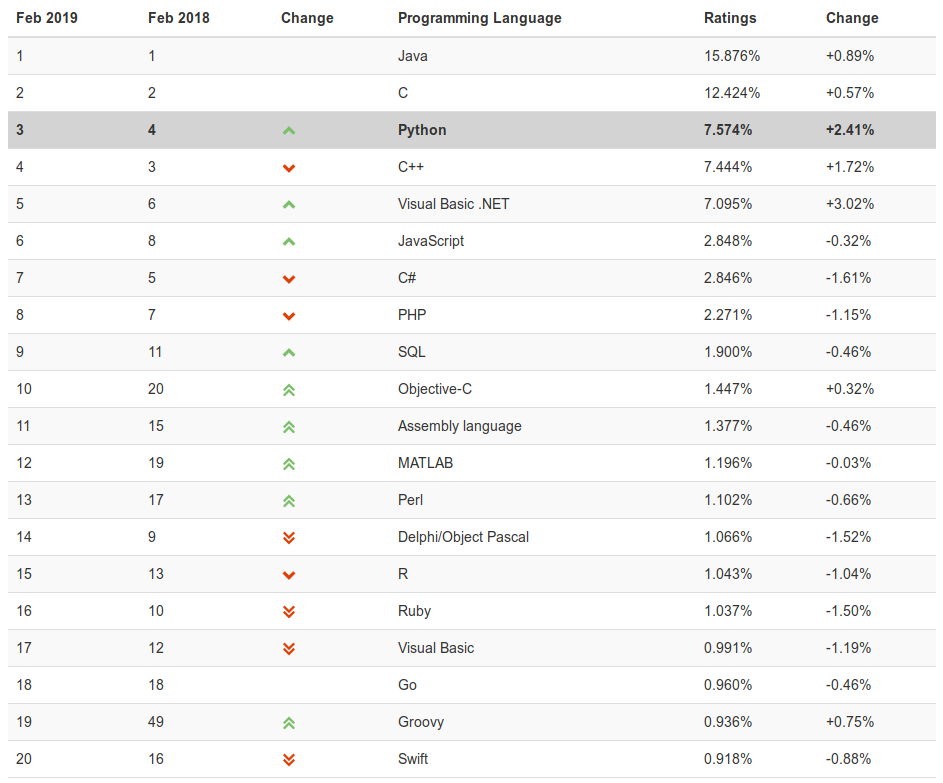
\includegraphics[width = 10cm]{TiobeIndex.png}
}



\frame{\frametitle{Python compared to other languages}
\rowcolors{1}{}{lightgray}
\begin{tabular}{c c c c c}
    & Python & C/C++ & Java & R 
\pause 
    \\ 
    Running speed & OK & Extremely fast & OK & Slow \pause \\  
    Easy to code? & Very easy & Extremely hard & Hard/OK & OK \pause \\  
    Portable? & Very easy & Hard & Very easy & Easy \pause \\  
    Documentation & Excellent & Very poor & Poor & Poor \pause \\  
\end{tabular}
}

\begin{frame}{Why do \textit{you} want to learn Python?}
    Some reasons:
    \pause
    \begin{itemize}
        \item As Python is simple, yet widely used, best programming language for starters
            \pause
        \item Easy to automate boring tasks (collecting data from multiple files, manipulating images, mining text data, etc)
            \pause
        \item Python and R are rapidly overtaking Perl as the main programming languages in Bioinformatics
            \pause
        \item Major GIS applications (e.g.,, ArcGIS) use Python as the main scripting language
            \pause
        \item Python is (far) easier to debug than R or C
    \end{itemize}
\end{frame}

\frame{\frametitle{Executing Python code}
\begin{enumerate}
    \item Use the Python IDLE interpreter (to test small pieces of code) 
    \item Executing python scripts written in a text editor (the main way to run Python code)
\end{enumerate}
}


\frame{\frametitle{Executing Python code I: the IDLE interpreter on Windows}
In the Windows start menu, go to the Python 3.XX folder and start the IDLE (Integrated Development and Learning Environment):\\
\begin{center}
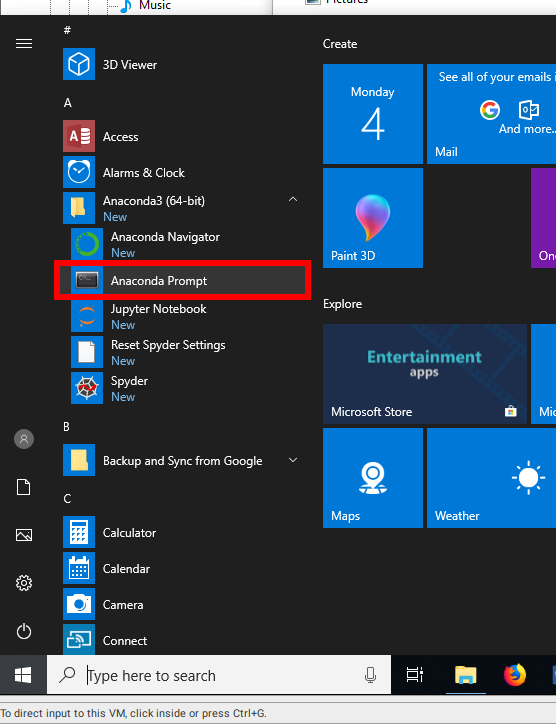
\includegraphics[width=0.3\textwidth]{WindowsStartIDLE.png}
\end{center}
}

\frame{\frametitle{Executing Python code I: the IDLE interpreter on Windows}
\begin{itemize}
    \item The IDLE interpreter will appear
    \item Any python code you type in is executed (and printed) once you type enter
\end{itemize}
\begin{center}
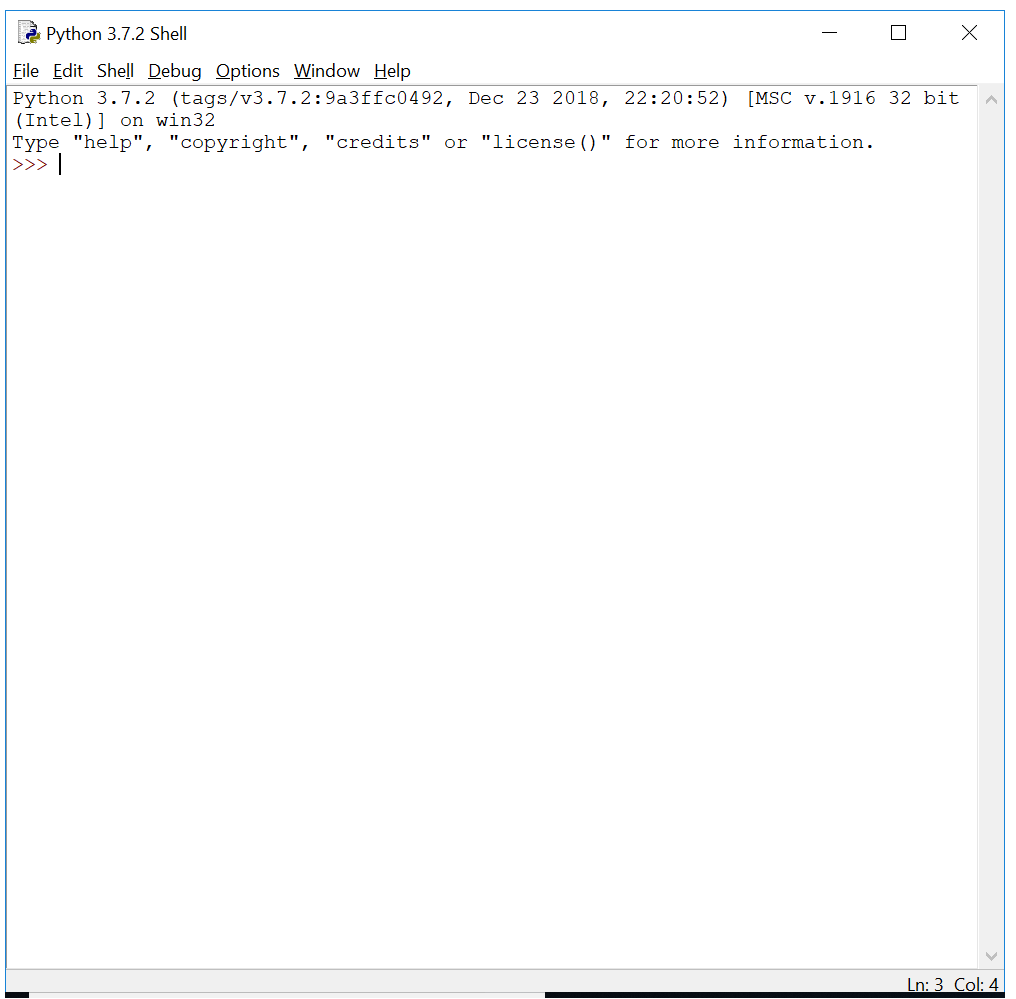
\includegraphics[width=0.5\textwidth]{WindowsPythonIDLE.png}
\end{center}
}

\frame{\frametitle{Executing Python code I: the IDLE interpreter on Mac}
\begin{itemize}
    \item Start a terminal by going to Applications $>$ Utilities $>$ Terminal
    \item Type \texttt{python3} (not \texttt{python}) to invoke the IDLE
    \item Any python code you type in is executed (and printed) once you type enter
\end{itemize}
\begin{center}
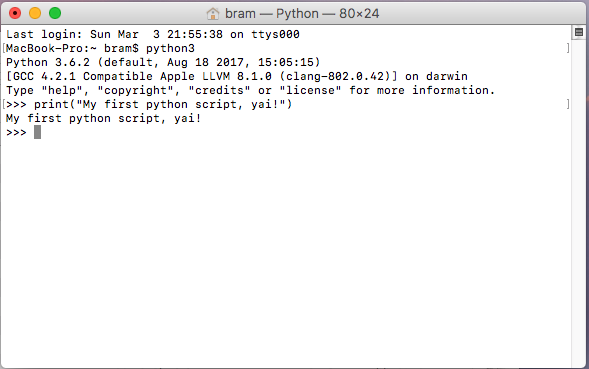
\includegraphics[width=0.5\textwidth]{MacPythonIDLE.png}
\end{center}
}

\frame{\frametitle{Invoking serious python scripts on Windows}
    
}

\end{document}

